%! Author = ibw
%! Date = 09.11.23

% Preamble

%Zusätzlich wurde eine \Gls{SWOT}-Analyse für das Projekt erstellt, um weitere Risiken und Gefahren für das Projekt aufzudecken.
%Dabei bezieht sich die Externe Betrachtung auf die Umsysteme und die ICT des KSGR und die Interne Betrachtung auf mich und das Team um mich herum.
%\begin{figure}[H]
%    \centering
%    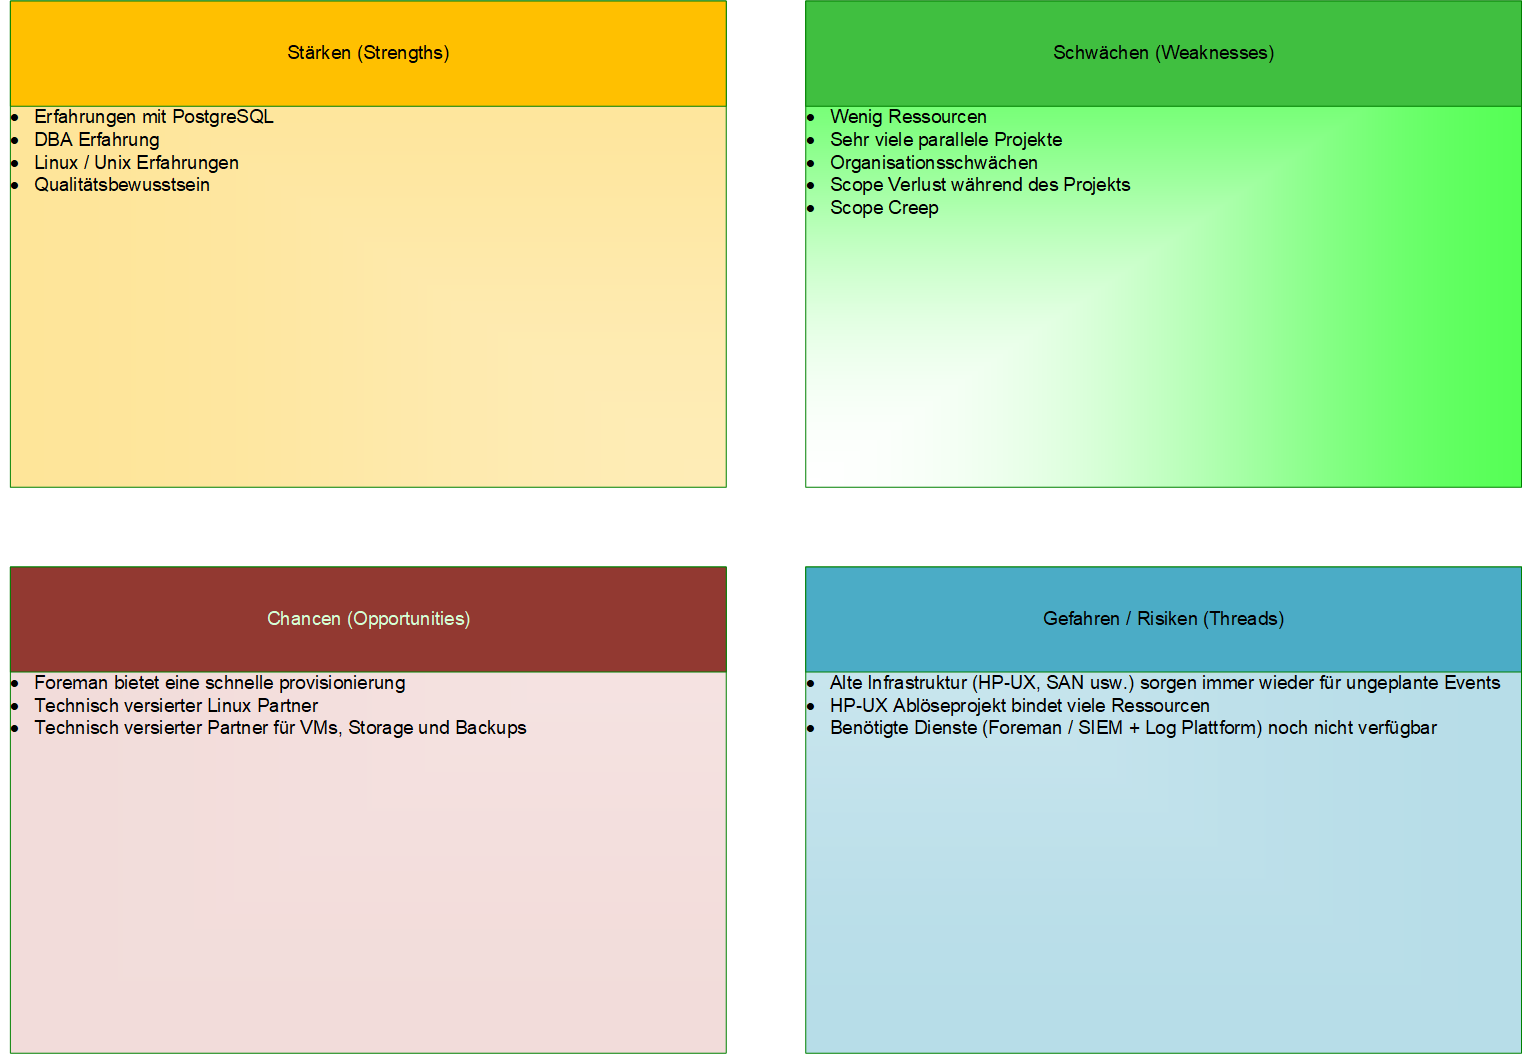
\includegraphics[width=1\linewidth]{source/introduction/riskmanagement/swot_projekt}
%    \caption{SWOT-Analyse Projekt}
%    \label{fig:swot-analysis-project}
%\end{figure}
\begin{landscape}
\begin{flushleft}
    \section{Risikomanagement}
    Aus den Abhängigkeiten heraus wurden folgende Risiken identifiziert:
\end{flushleft}
\begin{table}[H]
\resizebox{\columnwidth}{!}{%
\begin{tabular}{llllllllll}
\hline
\multicolumn{2}{l}{}                                                                                           &                                                                                                                                                                                                                                                    &                                                                                                                                                                                                                                                                                             & \multicolumn{2}{l}{}                                  & \multicolumn{4}{l}{Behandlung}                                                                                                                                                                             \\ \cline{7-10}
\multicolumn{2}{l}{\multirow{-2}{*}{Identifikation}}                                                           & \multirow{-2}{*}{}                                                                                                                                                                                                                                 & \multirow{-2}{*}{}                                                                                                                                                                                                                                                                          & \multicolumn{2}{l}{\multirow{-2}{*}{Abschätzung}}     &                                         & \multicolumn{2}{l}{Zielwert} &                                                                                                                                   \\ \cline{1-6} \cline{8-9}
ID & Risiko                                                                                                    & Beschreibung / Ursache                                                                                                                                                                                                                             & Auswirkung                                                                                                                                                                                                                                                                                  & WS                        & SM                        & \multirow{-2}{*}{Massnahmen ergreifen?} & WS            & SM           & \multirow{-2}{*}{Massnahme}                                                                                                       \\ \hline
1  & Fehlende Ressourcen                                                                                       & Viele parallele Projekte, Aufträge und der Tagesbetrieb                                                                                                                                                                                            & Ressourcen während der Diplomarbeit sind knapp bemessen                                                                                                                                                                                                                                     & \cellcolor[HTML]{F8FF00}3 & \cellcolor[HTML]{F8FF00}4 & Ja                                      & 2             & 2            & \begin{tabular}[c]{@{}l@{}}Organisation und\\ Selbstmanagement\end{tabular}                                                       \\
2  & \Gls{HP-UX} Ablöseprojekt                                                                                       & \begin{tabular}[c]{@{}l@{}}Das Projekt ist sehr Umfangreich\\ und ist in die Konzeptions- und Umsetzungsphase gestartet\end{tabular}                                                                                                               & \begin{tabular}[c]{@{}l@{}}Das Projekt wird parallel zur Diplomarbeit\\ sehr viele Ressourcen und Aufmerksamkeit binden\end{tabular}                                                                                                                                                        & \cellcolor[HTML]{F8FF00}4 & \cellcolor[HTML]{F8FF00}4 & Ja                                      & 3             & 3            & Ressourcen reservieren                                                                                                            \\
3  & \begin{tabular}[c]{@{}l@{}}Alte Infrastruktur kann\\ ungeplant sämtliche Ressourcen binden\end{tabular}   & \begin{tabular}[c]{@{}l@{}}\Gls{HP-UX} Plattform, DELL NetWorker / Data Domain Umgebung\\ und HPE 3PAR \Gls{SAN} Storage Umgebung sind über dem Lifecycle\\ und haben in den vergangenen Monaten immer wieder kritische Ausfälle erlebt\end{tabular}           & \begin{tabular}[c]{@{}l@{}}Bei einem Event, ausgelöst durch das Alter der \Gls{HP-UX} Plattform,\\ der DELL NetWorker / Data Domain Umgebung oder dem SAN Storage,\\ kann der ganze Betrieb zum erliegen kommen und entsprechend\\ viele Ressourcen aufgrund der kritikalität binden\end{tabular} & \cellcolor[HTML]{F8FF00}4 & \cellcolor[HTML]{F8FF00}4 & Ja                                      & 3             & 3            & \begin{tabular}[c]{@{}l@{}}Monitoring vorgängig ausbauen\\ und Massnahmen definieren\end{tabular}                                 \\
4  & \begin{tabular}[c]{@{}l@{}}Schwächen beim\\ Selbstmanagement und\\ in der Selbstorganisation\end{tabular} & Selbstmanagement und Organisation ist nicht meine Stärke                                                                                                                                                                                           & \begin{tabular}[c]{@{}l@{}}Das Projekt verzettelt sich, Zeit geht verloren.\\ Auch eine folge könnte der Scope Verlust sein\end{tabular}                                                                                                                                                    & \cellcolor[HTML]{F8FF00}3 & \cellcolor[HTML]{F8FF00}3 & Ja                                      & 2             & 2            & \begin{tabular}[c]{@{}l@{}}Werkzeuge im Vorfeld\\ definieren und bereitstellen\end{tabular}                                       \\
5  & Scope verlust während des Projekts                                                                        & Der Scope kann während des Projekts verloren gehen                                                                                                                                                                                                 & Verzettelung und Zeitverlust bis hin zu scheitern                                                                                                                                                                                                                                           & \cellcolor[HTML]{F8FF00}3 & \cellcolor[HTML]{F8FF00}4 & Ja                                      & 2             & 3            & Ziele klar definieren                                                                                                             \\
6  & Scope Creep                                                                                               & \begin{tabular}[c]{@{}l@{}}Der Umfang kann stark steigen wenn Ziele\\ nicht genau genug definiert wurden\end{tabular}                                                                                                                              & Zeitverlust bis hin zu scheitern des Projekts                                                                                                                                                                                                                                               & \cellcolor[HTML]{F8FF00}3 & \cellcolor[HTML]{F8FF00}4 & Ja                                      & 3             & 3            & Ziele SMART definieren                                                                                                            \\
7  & SIEM / Log Plattform nicht betriebsbereit                                                                 & \begin{tabular}[c]{@{}l@{}}Die öffentliche Ausschreibung für die neue   / Log\\ Plattform wurde erst am 23.10.2023 veröffentlicht.\\ Bis zur Implementation kann noch Zeit vergehen.\end{tabular}                                              & \begin{tabular}[c]{@{}l@{}}Logs müssen länger auf dem System selber vorgehalten werden.\\ Zudem müssen ggf. eigene Massnahmen zum\\ Auslesen von Logs getroffen werden\end{tabular}                                                                                                         & \cellcolor[HTML]{F8FF00}4 & 1                         & Nein                                    &               &              &                                                                                                                                   \\
8  & \Gls{Foreman} nicht betriebsbereit                                                                              & \begin{tabular}[c]{@{}l@{}}Die \Gls{Foreman} Provisioning- und Lifecycle Plattform\\ befindet sich aktuell erst in der Proof of Concept Phase.\\ Dadurch besteht das Risiko, dass sie nicht\\ betriebsbereit zum Start der Diplomarbeit ist\end{tabular} & \begin{tabular}[c]{@{}l@{}}Ms müssen von Hand provisioniert werden.\\ Dies bedeutet einen massiven Mehraufwand und verzögert\\ ggf. die Evaluationsphase und mit sicherheit die Installationsphase\end{tabular}                                                                             & 3                         & \cellcolor[HTML]{F8FF00}5 & Ja                                      & 3             & 4            & \begin{tabular}[c]{@{}l@{}}Massnahmen ergreifen um die manuelle\\ Installation so effizient wie möglich zu gestalten.\end{tabular} \\ \hline
\end{tabular}%
}
\caption{Risiko-Matrix der Diplomarbeit}
\label{tab:riskmatrix-projekt}
\end{table}
\end{landscape}
\begin{flushleft}
Daraus ergibt sich folgende Risikomatrix
\end{flushleft}
\begin{figure}[H]
    \centering
    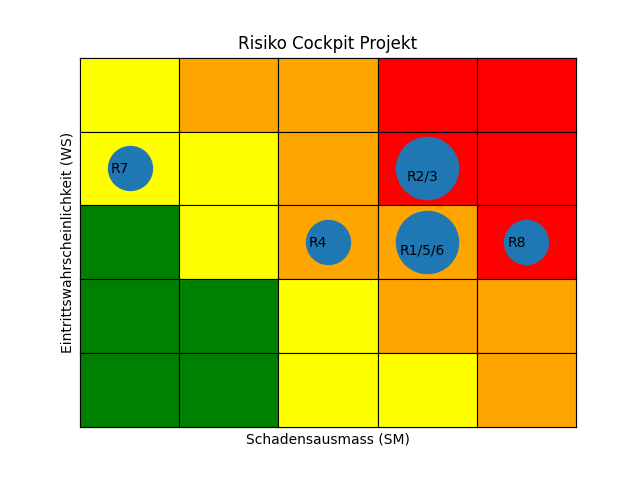
\includegraphics[width=0.75\linewidth]{source/riskmatrix/riskmatrix-project}
    \caption{Projektrisiken}
    \label{fig:riskmatrix-project}
\end{figure}
\begin{flushleft}
Mit den entsprechenden Massnahmen können die Risiken gesenkt werden:
\end{flushleft}
\begin{figure}[H]
    \centering
    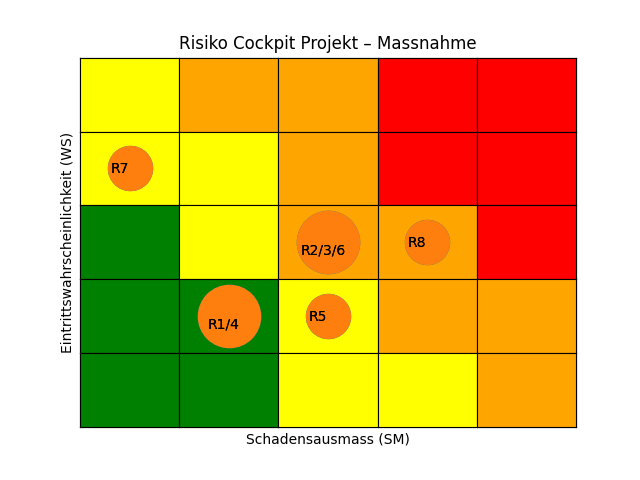
\includegraphics[width=0.75\linewidth]{source/riskmatrix/Riskmatrix-project-massnahmen}
    \caption{Projektrisiken mit Massnahmen}
    \label{fig:riskmatrix-project-massnahmen}
\end{figure}
